\subsection{Верхня оцінка відновлюючого спектрального числа для уніциклічного графа}
Для зваженого уніциклічного графа, розглянемо поставлену задачу. Для цього введемо теорему, на якій буде будуватися розв'язок.

\textbf{Теорема 4. [14]}\\
Нехай $F$ --- довільний зважений граф, $z\in V(F)$ та $H$ --- дерево з коренем $y$. Граф ${G}$ --- об'єднання графів $F,\ H$ та ребра, що з'єднує вершини $z$ та $y$. Тоді за спектрами \textbf{G} та всіх підграфів виду ${\bf G} - v$, де $v$ пробігає $CV(H)$ --- множина висячих вершин, можна відновити ваги на ребрах графа $\bf H$, вагу на ребрі $(z,y)$, а також $P_{\bf F}$,$P_{{\bf F}-\{z\}}$.\\

Знайдемо верхню оцiнку спектрального вiдновлюючого числа для уніциклічного графа.
Розглянемо перший випадок, $F=C_n$, і граф \textbf{G} --- уніциклічний, зображений на рисунку \ref{UniC2:image}.
\begin{figure}[H]
    \centering
    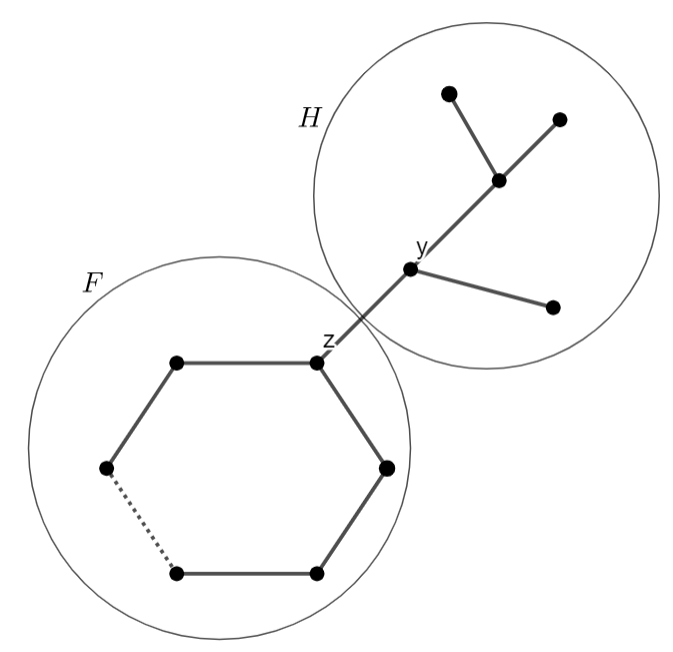
\includegraphics[width=0.4\linewidth]{pictures/UniC2.png}
    \caption{}
    \label{UniC2:image}
\end{figure}
За теоремою 4, ми відновлюємо ваги на ребрах графа $H$, вагу на ребрі $(z,y)$, а також $P_{\bf F}$,$P_{{\bf F}-\{z\}}$ за спектрами \textbf{G} та всіх підграфів виду ${\bf G} - v$, де $v$ пробігає $CV(H)$. Нам також необхідно відновити ваги не ребрах циклу. Оскільки ми знаємо характеристичний многочлен ланцюга $P_{{\bf F}-\{z\}}$, то знаючи характеристичний многочлен $P_{{\bf F}-\{z,u\}}$, де $u$ --- суміжна вершина з $z$, ми відновлюємо ваги усіх ребер, окрім тих, які є інцидентні з вершиною $z$. Отже, нам ще треба знати вагу одного з ребра, яке інцидентне з вершиною $z$ і ми зможемо відновити усі ваги графа \textbf{G}. Тобто для такого графа \textbf{G}(див. рисунок \ref{UniC2:image}) $Srn({G}) \leq cv(G)+3$, де $cv(G)$ --- кількість висячих вершин.

Розглянемо другий випадок, коли ми маємо декілька дерев $H_k$, що приєднані через ребро-міст і граф \textbf{G} --- уніциклічний, зображений на рисунку \ref{UniC3:image}.
\begin{figure}[H]
    \centering
    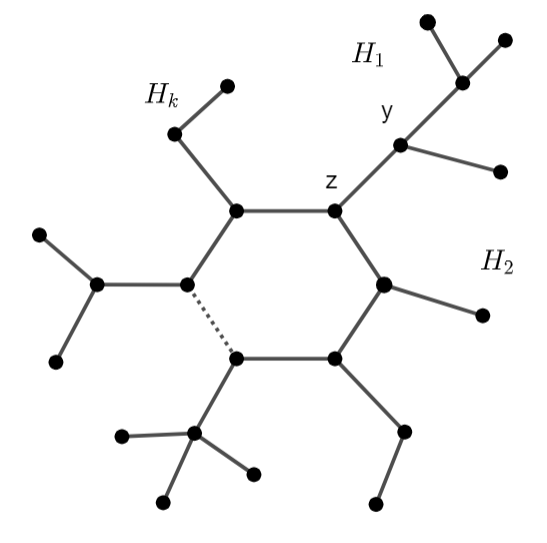
\includegraphics[width=0.4\linewidth]{pictures/UniC3.png}
    \caption{}
    \label{UniC3:image}
\end{figure}
Застосуємо теорему $k$ разів, тобто для кожного $F =  G - H_i$ і дерева $H_i$, $i \in 1,...,k$. Ми відновлюємо ваги на ребрах графів ${\bf H_1,...,H_k},\ k\in 1,...,n$, де $n$ --- кількість вершин у циклі, ваги на ребрах $(z_i,y_i)$, а також $P_{\bf F}$,$P_{{\bf F}-\{z_i\}}$ за спектрами \textbf{G} та всіх підграфів виду ${\bf G} - v$, де $v$ пробігає $CV(H) = CV(H_1) \cup ... \cup CV(H_k)$. Нам також необхідно відновити ваги не ребрах циклу, які ми точно можемо відновити знаючи ще 2 підспектри, що розписано у попередньому пункті. Тобто для такого графа \textbf{G}(див. рисунок \ref{UniC3:image}) $Srn({G}) \leq cv(G)+3$.

Розглянемо також третій випадок коли $F=C_n$, ми маємо декілька дерев $H_k$ і граф \textbf{G} --- уніциклічний, зображений на рисунку \ref{UniC5:image}.
\begin{figure}[H]
    \centering
    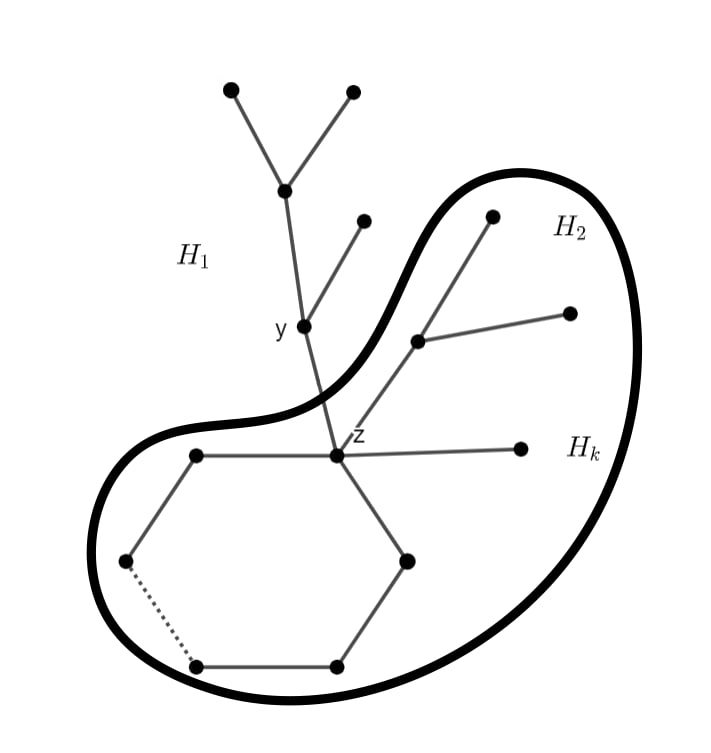
\includegraphics[width=0.4\linewidth]{pictures/UniC5.jpg}
    \caption{}
    \label{UniC5:image}
\end{figure}
Як і у попередньому випадку для кожного $F =  G - H_i$ і дерева $H_i$,\\ $i \in 1,...,k$, застосуємо теорему 4 і відновимо ваги на ребрах графів ${\bf H_1,...,H_k},\\ \ k\in \mathbf{N}$, ваги на ребрах $(z,y_i)$, а також $P_{\bf F}$,$P_{{\bf F}-\{z\}}$ за спектрами \textbf{G} та всіх підграфів виду ${\bf G} - v$, де $v$ пробігає $CV(H) = CV(H_1) \cup ... \cup CV(H_k)$. Нам також необхідно відновити ваги не ребрах циклу, які ми точно можемо відновити за двома підспектрами, що розписано у першому пункті. Тобто для такого графа \textbf{G}(див. рисунок \ref{UniC5:image}) $Srn({G}) \leq cv(G)+3$.

Отже, для довільного уніциклічного графа \textbf{G}: $Srn({G}) \leq cv({G})+3$.